%% chapter dedicated to the design of the prototype
\chapter{Prototype Design and Construction}

    \section{Technical Requirements}

        The main goal of the project is to create an interface between the ECU and the injectors that enables the use of alternative fuels by modifying the \gls{injection_pulse_width}. After careful consideration, the following technical requirements were set:

        \begin{itemize}
            \item \textbf{Power Supply:} Operation from a standard automotive 12V system (lead-acid battery).

            \item \textbf{Injection Detection:} Accurate detection of start of injection (SOI) and end of injection (EOI) signals from the ECU with precise measurement of the pulse width.

            \item \textbf{Pulse Width Extension:} Ability to extend the injector "ON" time by an adjustable percentage to accommodate different fuel requirements.

            \item \textbf{Installation:} Positioned between the ECU injector driver and the injector solenoid, completely isolating the injector from the ECU.

            \item \textbf{ECU Compatibility:} Emulation of the injector impedance characteristics to prevent detection by the ECU diagnostic systems.

            \item \textbf{Power Management:} Efficient dissipation or reuse of the injector power signal from the ECU.

            \item \textbf{Multi-cylinder Support:} Compatibility with various injection system configurations and firing orders, supporting up to 6 cylinders.

            \item \textbf{Injector Drive Control:} Support for Peak and Hold operation mode with adjustable peak time and PWM frequency for current control.
        \end{itemize}

    \section{System Architecture}

    
        %% insert figure with the block diagram of the system

        \begin{figure}[H]
            \centering
            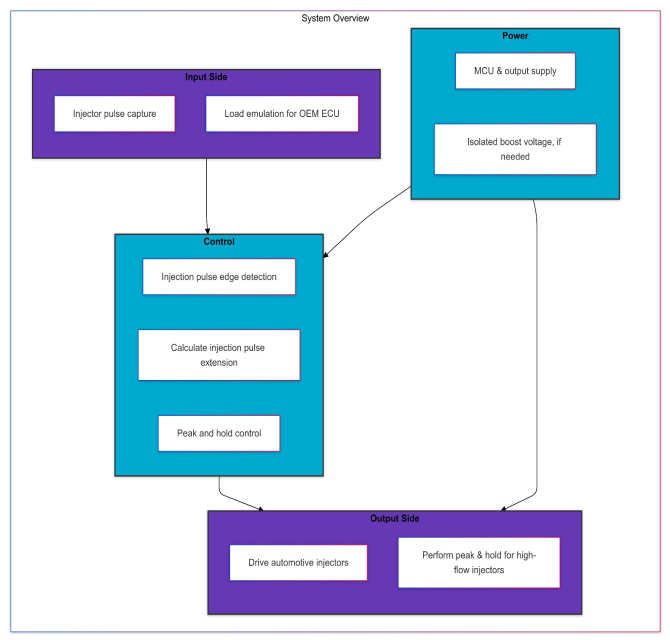
\includegraphics[width=0.8\textwidth]{system_block_diagram.png}
            \caption{Block Diagram of the Prototype System}
            \label{fig:block_diagram}
        \end{figure}

        The requirements above led to a design that can be split into 4 main functional groups:

        \begin{itemize}
            \item \textbf{Input Block:} Captures the \gls{soi} and \gls{eoi} signals from the ECU, ensuring accurate timing for pulse width measurement.
            \item \textbf{Power Management Block:} Manages the \gls{mcu} power supply and the injector driver power supply.
            \item \textbf{Control Block:} Unlike previous designs that have used a full analog approach to manipulating the \gls{injection_pulse_width}, this design uses a \gls{mcu} to control the pulse width extension, the current control, and all other parameters of the injection pulse. At the expense of higher complexity, this approach allows for much greater flexibility, which is essential for adapting the module for different injection systems.
            \item \textbf{Output Block:} As complete isolation between the \gls{ecu} and the injectors is required, the module must also have the necessary hardware to drive injectors. This is realized by a peak and hold capable injector driver.
        \end{itemize}

        \subsection{Input Block}
            
            %% include figure the input block diagram picture

            \begin{figure}[H]
                \centering
                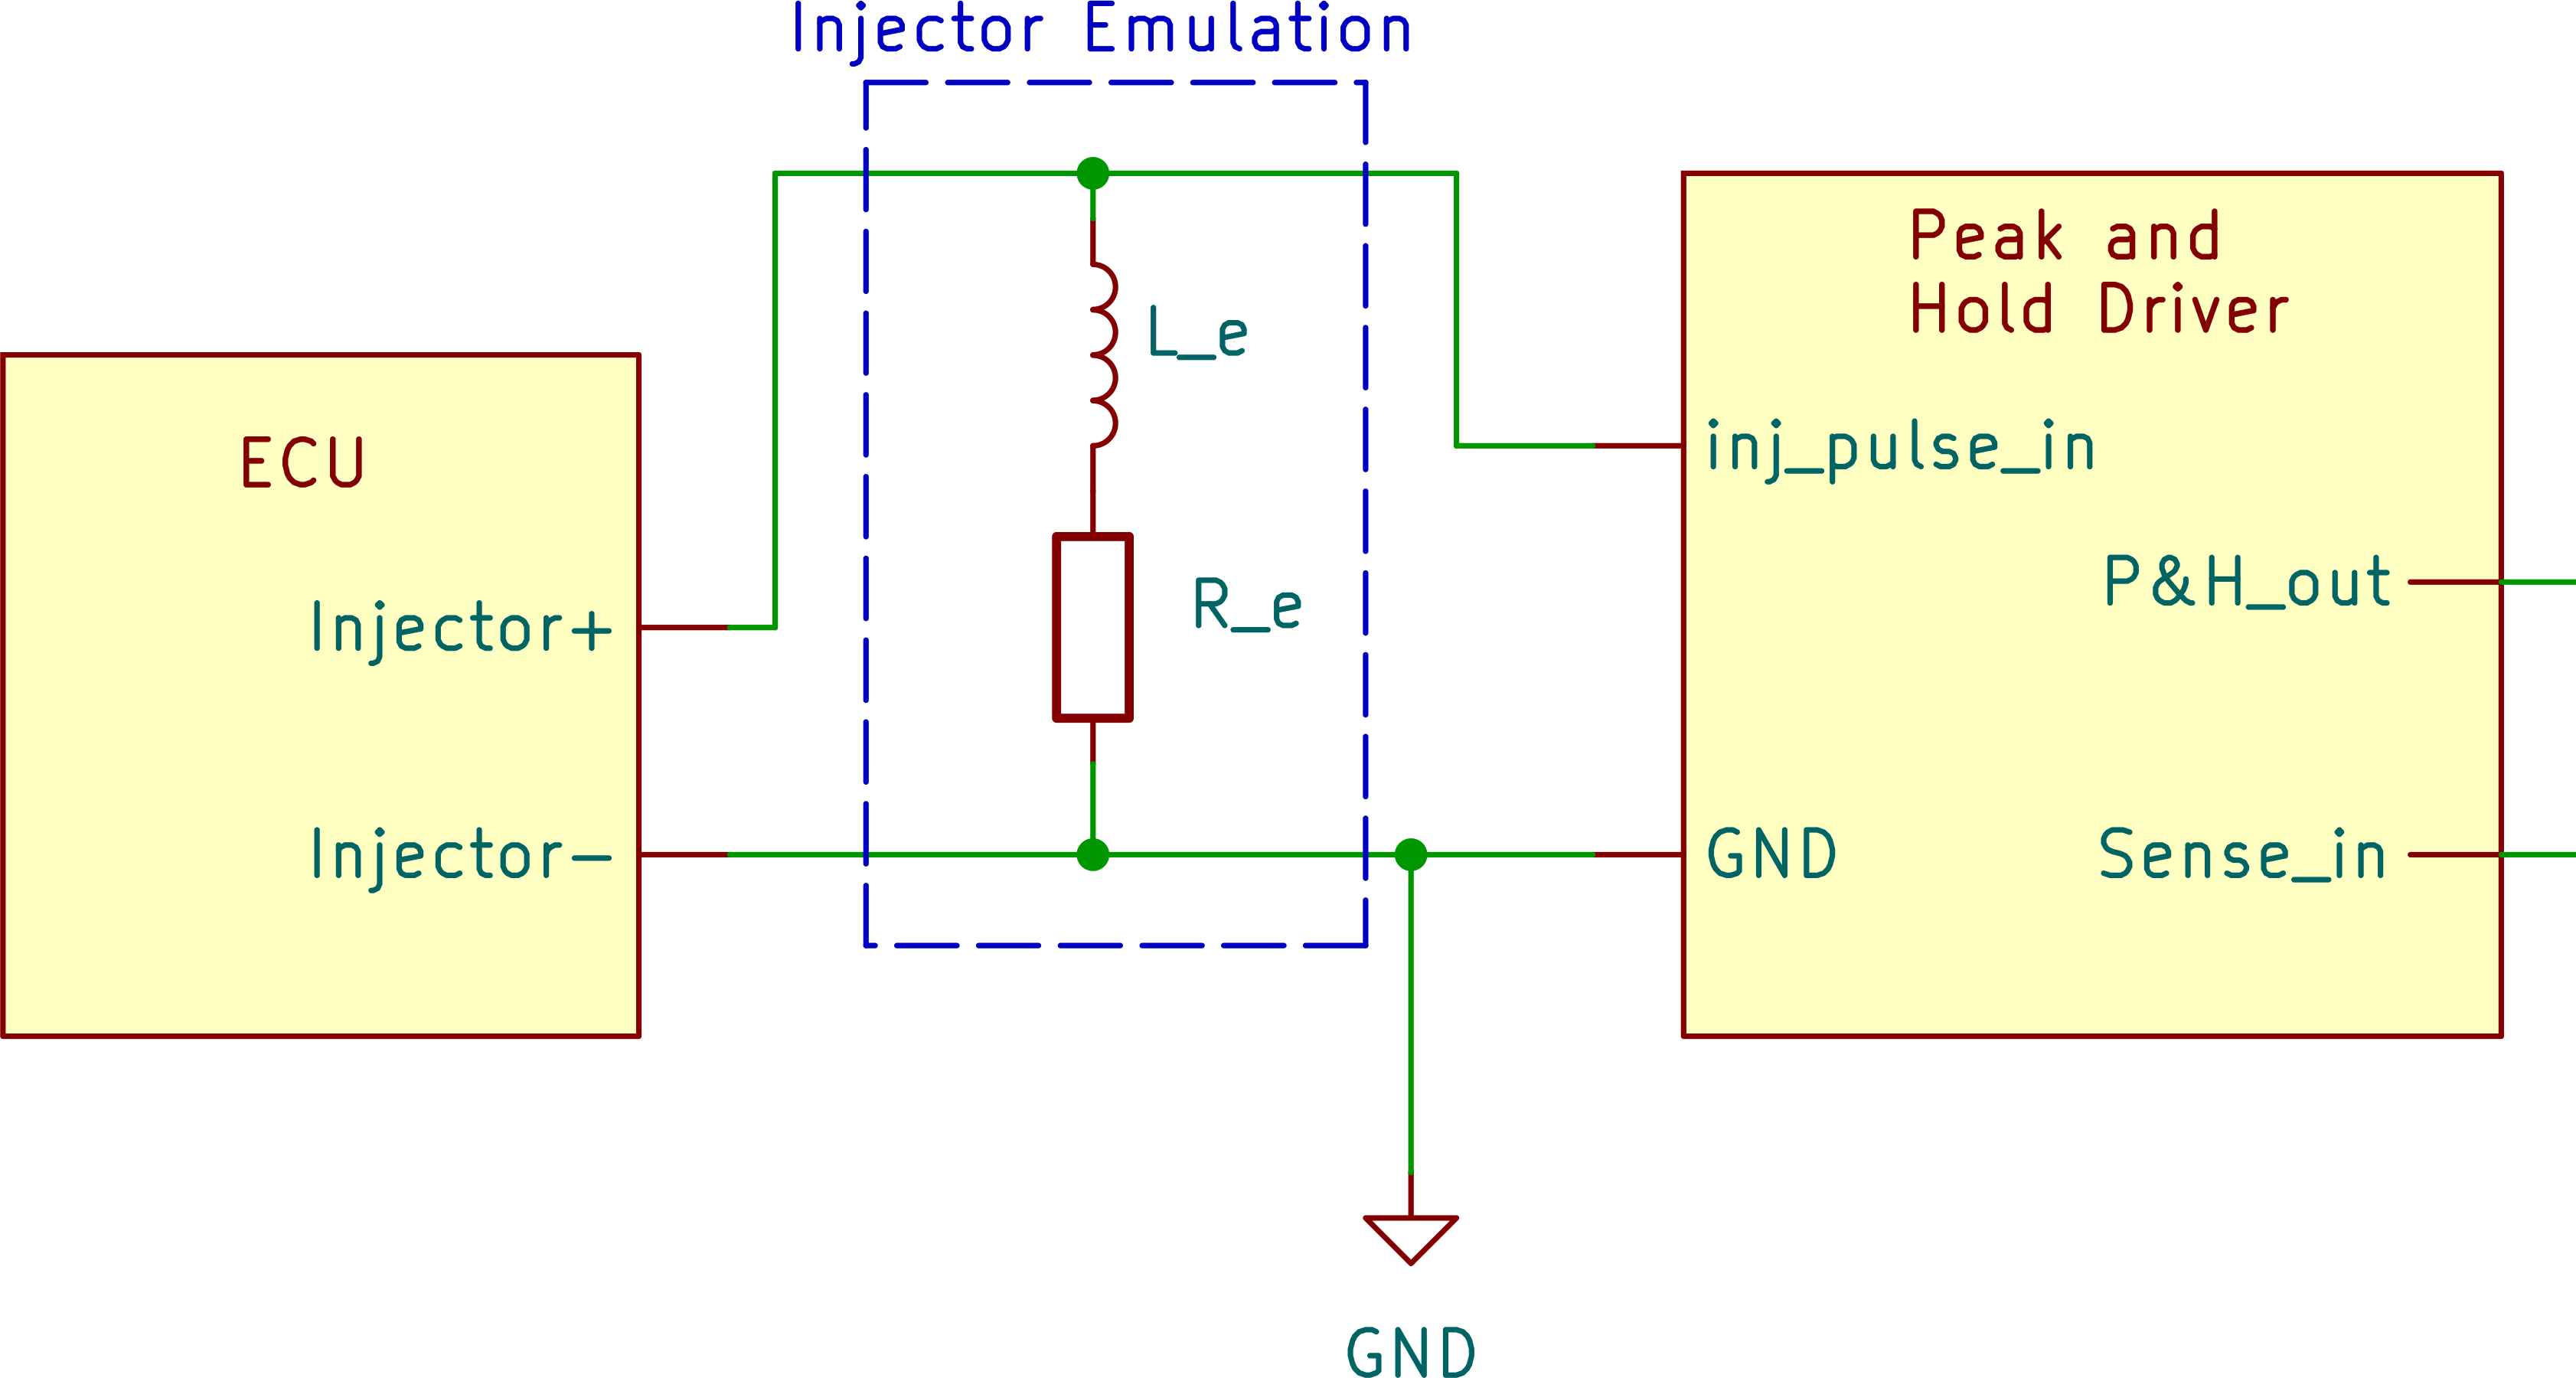
\includegraphics[width=0.8\textwidth]{input_side.png}
                \caption{Input Block Diagram}
                \label{fig:input_block_diagram}
            \end{figure}

            %% not sure which paragraph to use here

            %The main function of the input block is emulating the injector impedance characteristics to prevent errors from the \gls{ecu}. After testing on the Weber motor, it was found that a simple resistance of the same value as the injector DC impedance works well. Further study of other \gls{ecu}s would be needed to generalize this solution, but it is a good starting point.

            The main function of the input block is emulating the injector impedance for the \gls{ecu}. Different \gls{ecu}s have different diagnostics for injector parameters, and no solution can be guaranteed without testing on the specific version of the \gls{ecu}. For the Continental Easy - U1 WEBER \gls{ecu}, the initial plan was to emulate the injector impedance with a resistor and an inductor in series, to achieve a similar impedance curve to that of the injector. However, upon testing, it was found that a simple 12 $\Omega$ resistor is sufficient to prevent errors. Further testing is necessary to evaluate if this is a long-term solution, and if it could be generalized for other \gls{ecu}s.

            In any case, the power from the \gls{ecu} injector driver must be dissipated or reused. For this proof of concept prototype, a simple power resistor will be used to dissipate the power as heat, but future designs could use a more efficient solution to reuse the power.

        \subsection{Power Management Block}

            To simplify the design, it was decided to use the 12V battery power to supply the MOSFETs and the respective MOSFET drivers. For the microcontroller, a 12V to 3.3V step-down converter was used. The microcontroller can also be powered through USB, greatly simplifying the first prototype. Special care has to be taken against the reverse polarity of the power supply, as other typical hazardous situations in automotive applications (ISO 16750-2 and ISO 7637-2 describe several conditions that can lead to electrical failure in such an environment). Fuses and \gls{tvs} diodes are used to protect the circuit from some of these events.

            The \gls{tvs} diode provides a low impedance path to ground for any voltage spikes, protecting both the logic inputs and the power terminals of the components from overvoltage.

            %% Insert figure showing the \gls{tvs} diodes
            \begin{figure}[H]
                \centering
                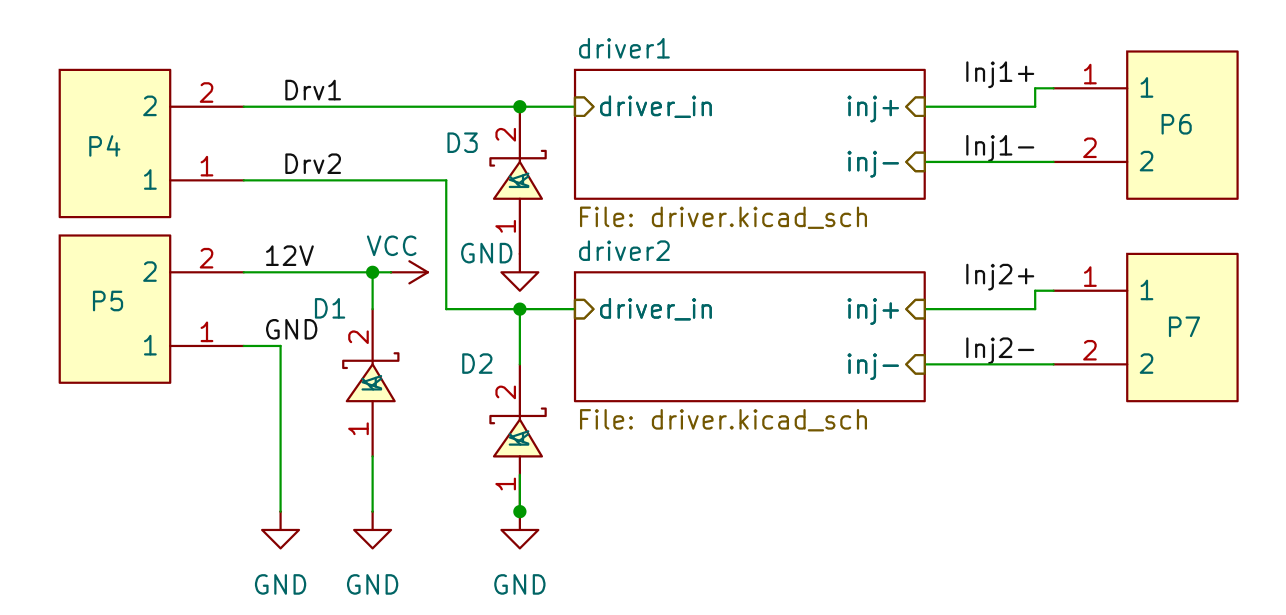
\includegraphics[width=1.0\textwidth]{tvs_protection.png}
                \caption{\gls{tvs} Diode protection on logic inputs and power terminals}
                \label{fig:tvs_protection}
            \end{figure}

            In the future, the input side can be combined with the power block to reuse the power from the \gls{ecu} injector driver, improving overall efficiency.

        \subsection{Control Block}

            The digital logic is realized through an ARM Cortex-M4 microcontroller, which handles the timing of the \gls{injection_pulse_width} 

            The logic can be summed up as follows:

            %% insert png image with flowchart
            \begin{figure}[H]
                \centering
                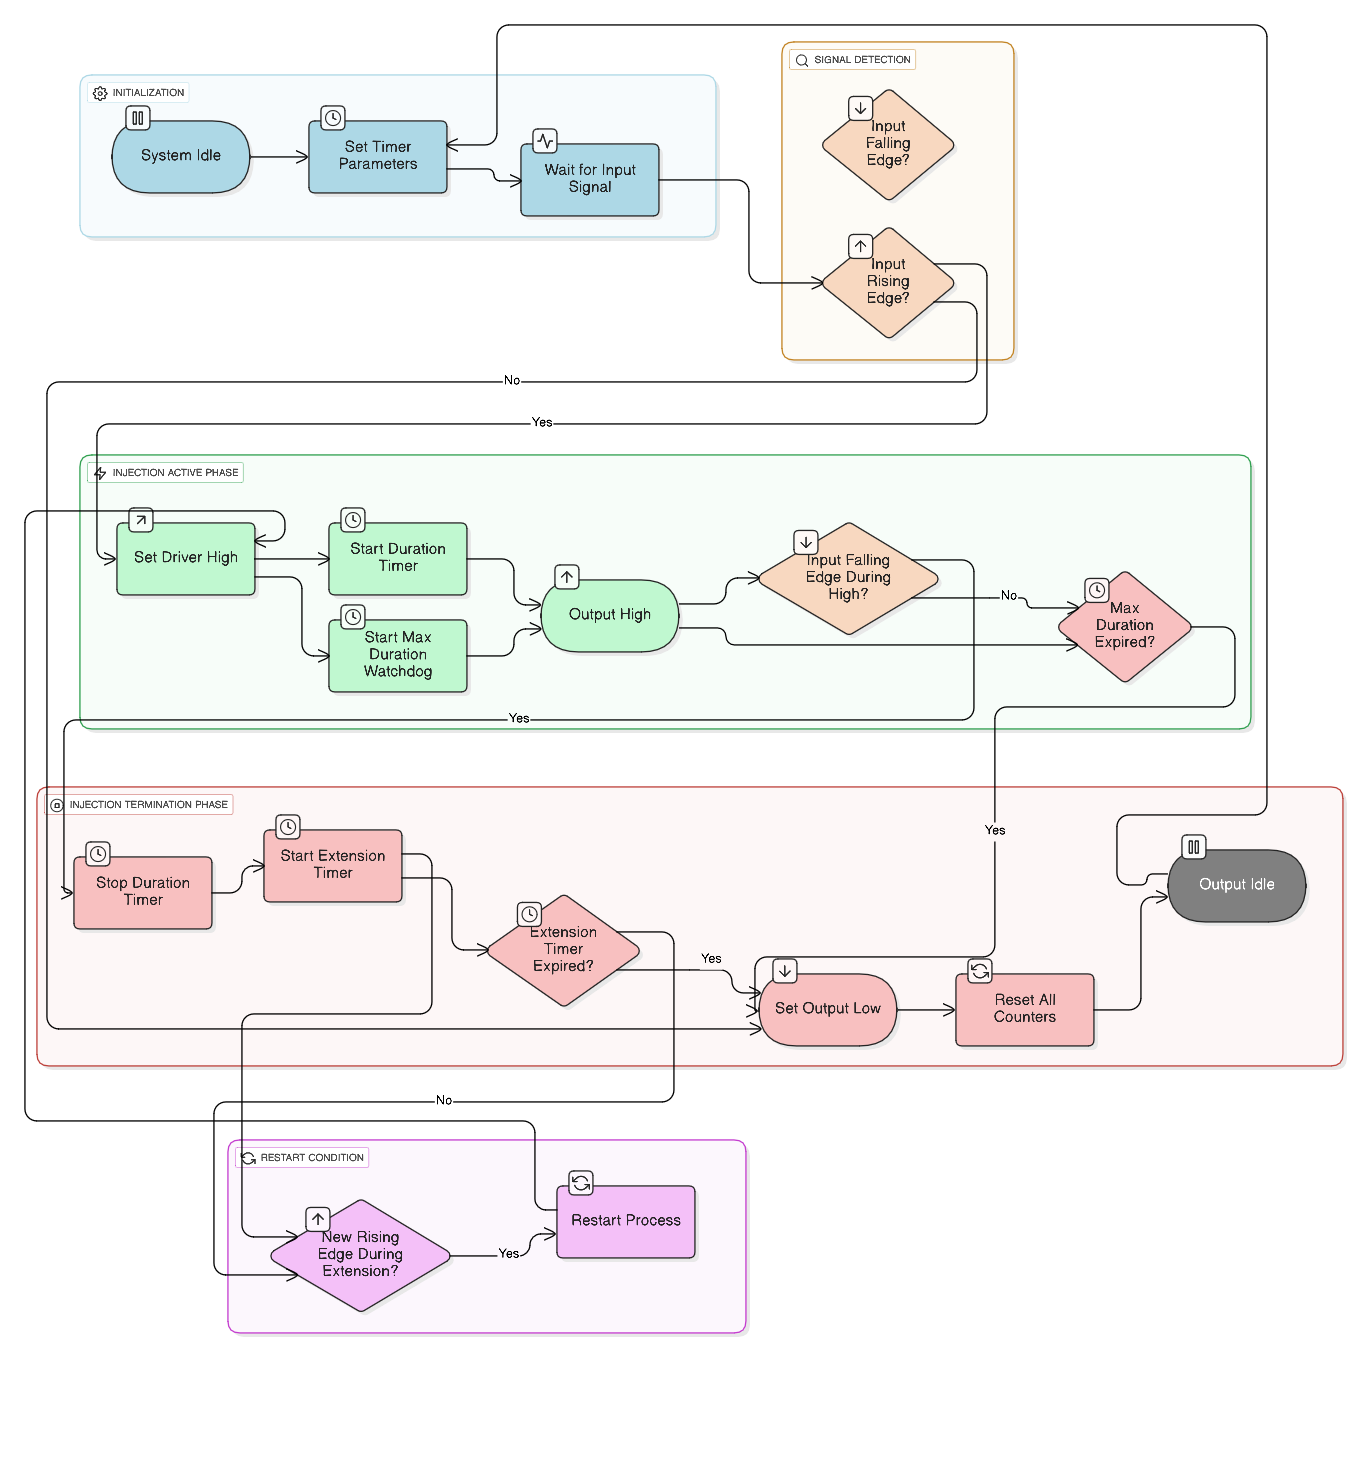
\includegraphics[width=1\textwidth]{flowchart_white.png}
                \caption{Control Logic Flowchart}
                \label{fig:control_logic_flowchart}
            \end{figure}

            The Cortex-M4 was chosen for its good clock speed, abundant peripherals, and most importantly, multiple timers. The digital logic was implemented in C, with focus on real-time performance, with a \gls{deterministic} approach. At 7000 RPM, each crank rotation takes approximately 8.57 ms, which means on a four-stroke engine, only 4.3 ms are available for the fuel to be injected. This is the so-called "injection window". At wide open throttle, the injector uses almost the entire injection window, up to 4.0 ms to inject fuel. The system must be able to react to an input fast enough to ensure that the injection still takes place inside the injection window.

            All core functionalities run on timer interrupts. With the detection of an injection event, a series of timers are started to control the injection process, and the peak and hold functionality, along with fail-safes to prevent catastrophic failure. This highly \gls{deterministic} approach is essential for an application like this.

            Several failure cases were considered, the most dangerous being pre-ignition of the mixture due to badly timed injection events, and uncontrolled injection, leading to the "flooding" of the cylinder.

            The latter could lead to the cylinder being filled with fuel while the motor is still off, and "lifting" the cylinder head when starting the motor (phenomenon known as "\gls{hydraulic_lock}"). To prevent this, the module has a failsafe that will stop the injection process if the \gls{injection_pulse_width} exceeds a certain threshold (see Figure \ref{fig:control_logic_flowchart}), which can be adjusted by the user. The code was also written in a manner that the output is normally low (that is, default output state is low).

            A failure to detect and react to an \gls{ecu} input in time could also lead to incomplete combustion, not giving the fuel time to undergo \gls{atomization} properly. The bare-metal timer approach allows for a highly \gls{deterministic} execution time, which minimizes the risks of this happening.

            %% \begin{figure}[H]
            %%     \centering
            %%     \begin{tikzpicture}[
            %%         node distance=0.4cm,
            %%         box/.style={rectangle, draw, minimum width=2cm, minimum height=0.6cm, text centered, rounded corners, font=\footnotesize},
            %%         oval/.style={ellipse, draw, minimum width=1.8cm, minimum height=0.6cm, text centered, font=\footnotesize},
            %%         diamond/.style={diamond, draw, minimum width=2cm, minimum height=0.8cm, text centered, font=\footnotesize},
            %%         arrow/.style={->,>=stealth, thin}
            %%     ]
            %%     
            %%     %% Initialization - More compact vertical layout
            %%     \node[oval, fill=blue!10] (idle) at (0,0) {System Idle};
            %%     \node[box, below=0.3cm of idle, fill=blue!10] (set_params) {Set Timer Parameters};
            %%     \node[box, below=0.3cm of set_params, fill=blue!10] (wait) {Wait for Input Signal};
            %%     
            %%     %% Signal Detection - Reduced horizontal spacing
            %%     \node[shape=diamond, right=1.5cm of wait, fill=orange!20] (rising) {Input Rising Edge?};
            %%     
            %%     %% Active Phase - Reduced spacing
            %%     \node[box, right=1.5cm of rising, fill=green!20] (driver_high) {Set Driver High};
            %%     \node[box, below=0.3cm of driver_high, fill=green!20] (start_timer) {Start Duration Timer};
            %%     \node[box, below=0.3cm of start_timer, fill=green!20] (start_watchdog) {Start Max Duration WD};
            %%     \node[oval, below=0.3cm of start_watchdog, fill=green!20] (output_high) {Output High};
            %%     \node[shape=diamond, below=0.3cm of output_high, fill=orange!20] (falling_during) {Input Falling Edge?};
            %%     \node[shape=diamond, right=1.5cm of falling_during, fill=red!20] (max_duration) {Max Duration Expired?};
            %%     
            %%     %% Termination Phase - More compact
            %%     \node[box, below=0.3cm of falling_during, fill=red!20] (stop_timer) {Stop Duration Timer};
            %%     \node[box, below=0.3cm of stop_timer, fill=red!20] (start_extension) {Start Extension Timer};
            %%     \node[shape=diamond, below=0.3cm of start_extension, fill=red!20] (extension_expired) {Extension Timer Expired?};
            %%     \node[box, below=0.3cm of extension_expired, fill=red!20] (output_low) {Set Output Low};
            %%     \node[box, below=0.3cm of output_low, fill=red!20] (reset_counters) {Reset All Counters};
            %%     \node[oval, below=0.3cm of reset_counters, fill=gray!20] (output_idle) {Output Idle};
            %%     
            %%     %% Restart Condition - Reduced spacing
            %%     \node[shape=diamond, right=1.5cm of start_extension, fill=purple!20] (new_rising) {New Rising Edge?};
            %%     \node[box, below=0.3cm of new_rising, fill=purple!20] (restart) {Restart Process};
            %%     
            %%     %% Arrows - Main Flow
            %%     \draw[arrow] (idle) -- (set_params);
            %%     \draw[arrow] (set_params) -- (wait);
            %%     \draw[arrow] (wait) -- (rising);
            %%     \draw[arrow] (rising) -- node[above, font=\scriptsize] {Yes} (driver_high);
            %%     \draw[arrow] (driver_high) -- (start_timer);
            %%     \draw[arrow] (start_timer) -- (start_watchdog);
            %%     \draw[arrow] (start_watchdog) -- (output_high);
            %%     \draw[arrow] (output_high) -- (falling_during);
            %%     \draw[arrow] (falling_during) -- node[left, font=\scriptsize] {Yes} (stop_timer);
            %%     \draw[arrow] (falling_during) -- node[above, font=\scriptsize] {No} (max_duration);
            %%     \draw[arrow] (max_duration) |- node[right, font=\scriptsize] {Yes} (output_low);
            %%     \draw[arrow] (stop_timer) -- (start_extension);
            %%     \draw[arrow] (start_extension) -- (extension_expired);
            %%     \draw[arrow] (start_extension) -- (new_rising);
            %%     \draw[arrow] (extension_expired) -- node[left, font=\scriptsize] {Yes} (output_low);
            %%     \draw[arrow] (extension_expired) -| node[below, font=\scriptsize] {No} (new_rising);
            %%     \draw[arrow] (new_rising) -- node[left, font=\scriptsize] {Yes} (restart);
            %%     \draw[arrow] (output_low) -- (reset_counters);
            %%     \draw[arrow] (reset_counters) -- (output_idle);
            %%     \draw[arrow] (output_idle) -| (idle);
            %%     \draw[arrow] (restart) -| (driver_high);
            %%     \draw[arrow] (rising) -| node[above, font=\scriptsize] {No} (wait);
            %%     
            %%     %% Add text labels with smaller font
            %%     \node[font=\footnotesize] at (0,-0.7) {Initialization};
            %%     \node[font=\footnotesize] at (1.5,-0.7) {Signal Detection};
            %%     \node[font=\footnotesize] at (3.5,-0.7) {Injection Active};
            %%     \node[font=\footnotesize] at (2,-3.5) {Termination Phase};
            %%     \node[font=\footnotesize] at (5,-3.5) {Restart Logic};
            %%     
            %%     \end{tikzpicture}
            %%     \caption{Flowchart of Injection Control Logic}
            %%     \label{fig:injection_control_flow}
            %% \end{figure}

    \section{Output Block}

        The output block design is, from a hardware point of view, the most critical part of the system, as it has to handle the high injector currents and the high kickback voltage resulting from the inductance of the injector.

        The output block was designed independently from the control block, to improve flexibility. Each output module has two injector outputs, and they can be used in parallel with a single control block to drive as many injectors as the control module can handle. 
        
        The output injector driver circuit is also driven directly from the 12V battery system, which negates the need for more power blocks when adding more output modules. This results in a fully modular system, that can be expanded to accommodate different injection system requirements.

        To achieve peak and hold operation, there are several approaches that can be used. A dual voltage supply can be used, with a high voltage to achieve the peak current, and a lower voltage for the hold phase. This, however, adds complexity, as it requires a boost converter for the high voltage, and a stepdown for the hold voltage.

        Another approach is to use a peak and hold driver IC, such as the Texas Instruments LM1949 \autocite{texasinstrumentsLM1949InjectorDrive1995}, which is designed specifically for this purpose.

        %% include picture of the LM1949 application circuit

        \begin{figure}[H]
            \centering
            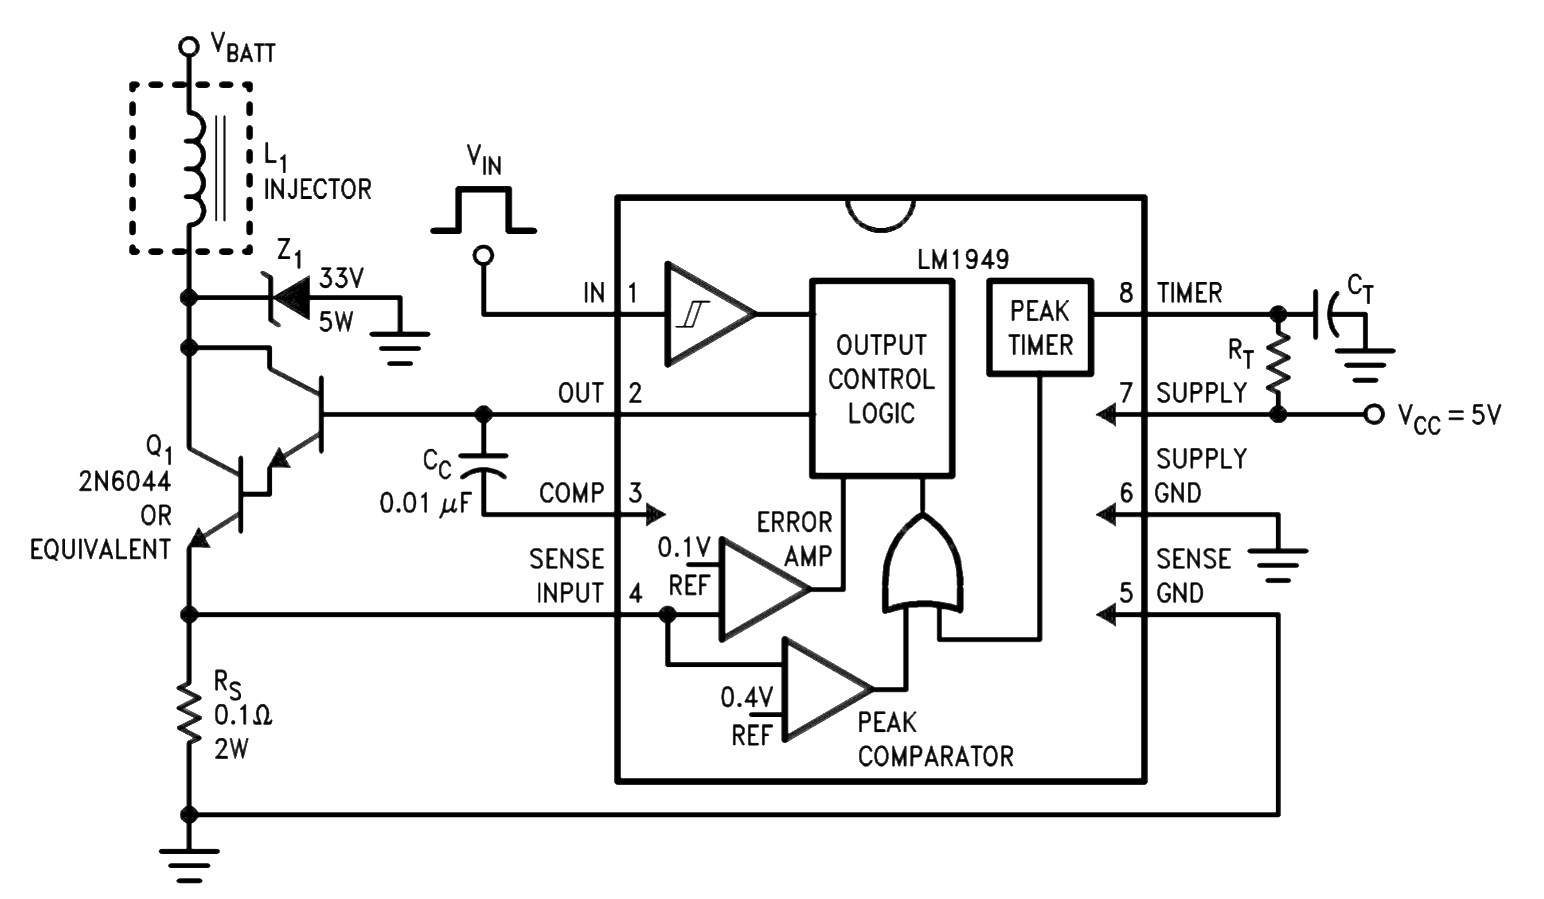
\includegraphics[width=0.8\textwidth]{lm1949_application.png}
            \caption{LM1949 Application Circuit. Adapted from \autocite{texasinstrumentsLM1949InjectorDrive1995}}
            \label{fig:LM1949_application_circuit}
        \end{figure}

        The LM1949, however, relies on a transistor operating in its linear region for the current control. This leads to high power dissipation and unnecessary losses on the driver. It can also be operated in a PWM mode, but this requires the PWM parameters to be set on a hardware level, which goes against the design philosophy of keeping the module as flexible as possible.

        For this sake, it was decided upon a custom peak and hold driver, which uses a low side N-channel power MOSFET to control the injector current. The current control is realized through a high frequency PWM signal, which is generated by the \gls{mcu} PWM timers. This simplified digital logic approach allows for maximum flexibility, as the PWM parameters can be adjusted in real-time through the \gls{mcu}.

        The circuit was also designed to be normally open, that is, the output will be low by default, so in case of failure, the output will be low, which means the injectors stay closed. \gls{tvs} diodes are also used to protect the input from overvoltage spikes, as well as the \gls{mcu} from the inductive kickback. A voltage follower circuit was also added to the \gls{mcu} outputs to guarantee isolation between logic and power circuits, preventing the high currents from affecting the \gls{mcu} operation.

        Later, input optical isolation had to be added to the circuit. The "Easy - U1 WEBER" \gls{ecu} uses an isolated ground for the injectors, not connected to the battery ground. This means that the input signals from the \gls{ecu} must be isolated from the output signals to prevent ground loops and ensure proper operation. An optocoupler was added to the input side of the circuit to provide this isolation, at the cost of increased complexity and latency (in the microsecond range, still very tolerable for the application).


        \subsection{Current Control}
           
            When switching a voltage across an inductor, if the switching frequency is high enough, the current will be constant, and controlled by the duty cycle of the PWM signal.

            %% prove this with equations
            If the voltage is switched on and off at a high frequency, the average current can be controlled by the duty cycle \(D\) of the PWM signal:
            \begin{equation}
                I_{avg} = D \cdot \frac{V}{R}
            \end{equation}
            where \(R\) is the resistance of the inductor.

            The so-called "hold" current, that is, the minimum current to hold the solenoid open, should be measured on an experimental basis for each injector type. 

            The peak current should be set to a value that is high enough to open the solenoid consistently.

            Due to the lack of data on the injectors on the Weber motor, and the lack of an adequate dedicated injector testbench to evaluate their performance, it was decided to drive the injectors on the Weber motor in saturation mode, just like the \gls{oem} \gls{ecu} does.


        \subsection{Kickback Protection}

            When the current through an inductor is suddenly interrupted, the inductor will try to maintain the current flow, leading to a voltage spike given by:
            \begin{equation}
                V_{kickback} = L \cdot \frac{di}{dt}
            \end{equation}
            where \(L\) is the inductance of the load and \(\frac{di}{dt}\) is the rate of change of current.

            This voltage spike is called inductive kickback, and can damage driving circuitry if not mitigated. The simple way to dissipate this energy is to provide a low impedance path to ground for the current to flow when the MOSFET is turned off. Two main solutions were considered: a freewheeling diode clamp and a Zener diode clamp.


            \subsubsection{Freewheeling Diode}

                The simplest approach is to use a freewheeling diode, which provides a path for the current to flow when the MOSFET is turned off. This diode should be rated for the maximum current and power dissipation of the injector.

                \begin{figure}[H]
                    \centering
                    \begin{subfigure}{0.25\textwidth}
                        \centering
                        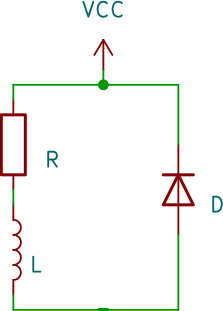
\includegraphics[width=\textwidth]{single_diode_std.png}
                        \caption{Freewheeling diode circuit schematic}
                        \label{fig:freewheeling_circuit}
                    \end{subfigure}
                    \hfill
                    \begin{subfigure}{0.7\textwidth}
                        \centering
                        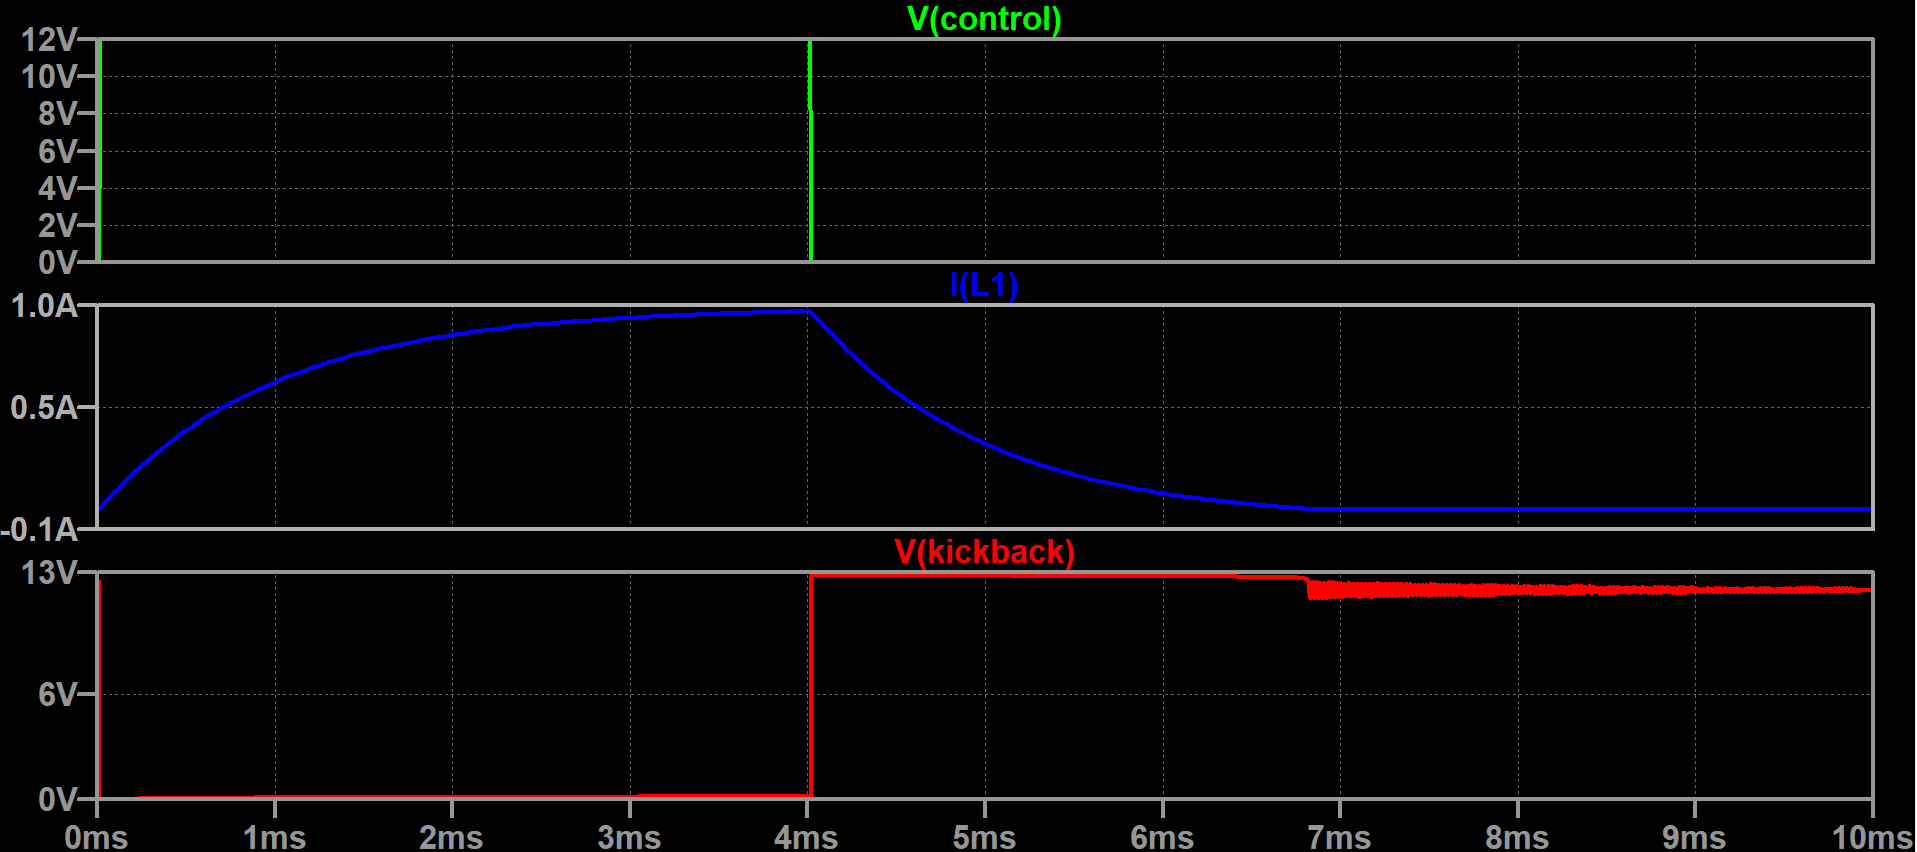
\includegraphics[width=\textwidth]{single_diode_sim_results.png}
                        \caption{Simulated waveforms showing inductor current and voltage}
                        \label{fig:freewheeling_waveform}
                    \end{subfigure}
                    \caption{Freewheeling diode implementation for inductive kickback protection. The diode provides a path for the current to flow when the MOSFET switches off, limiting the voltage spike across the inductor.}
                    \label{fig:freewheeling_combined}
                \end{figure}


            \subsubsection{Zener Clamp}

                A disadvantage of the simple freewheeling diode is that due to the low forward voltage of the diode and the internal resistance of the solenoid, the dissipation current will be very limited. For an injector with $12$ $\Omega$ of DC resistance, and a forward voltage of $0.7$ V, the current will be limited to approximately $0.06$ A, which is not enough to quickly dissipate the energy stored in the inductor. This results in a slow decay of the current, which increases the shutoff time of the injector. 

                Adding a Zener diode in series with the freewheeling diode can help to increase the voltage drop across the diodes, while still protecting the MOSFET from too high voltages. The Zener diode will clamp the voltage spike to a safe level, allowing the current to flow through the freewheeling diode and dissipate the energy stored in the solenoid as quickly as possible.

                \begin{figure}[H]
                    \centering
                    \begin{subfigure}{0.25\textwidth}
                        \centering
                        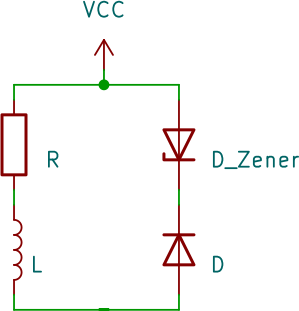
\includegraphics[width=\textwidth]{zener_diode_std.png}
                        \caption{Zener diode circuit schematic}
                        \label{fig:zener_circuit}
                    \end{subfigure}
                    \hfill
                    \begin{subfigure}{0.7\textwidth}
                        \centering
                        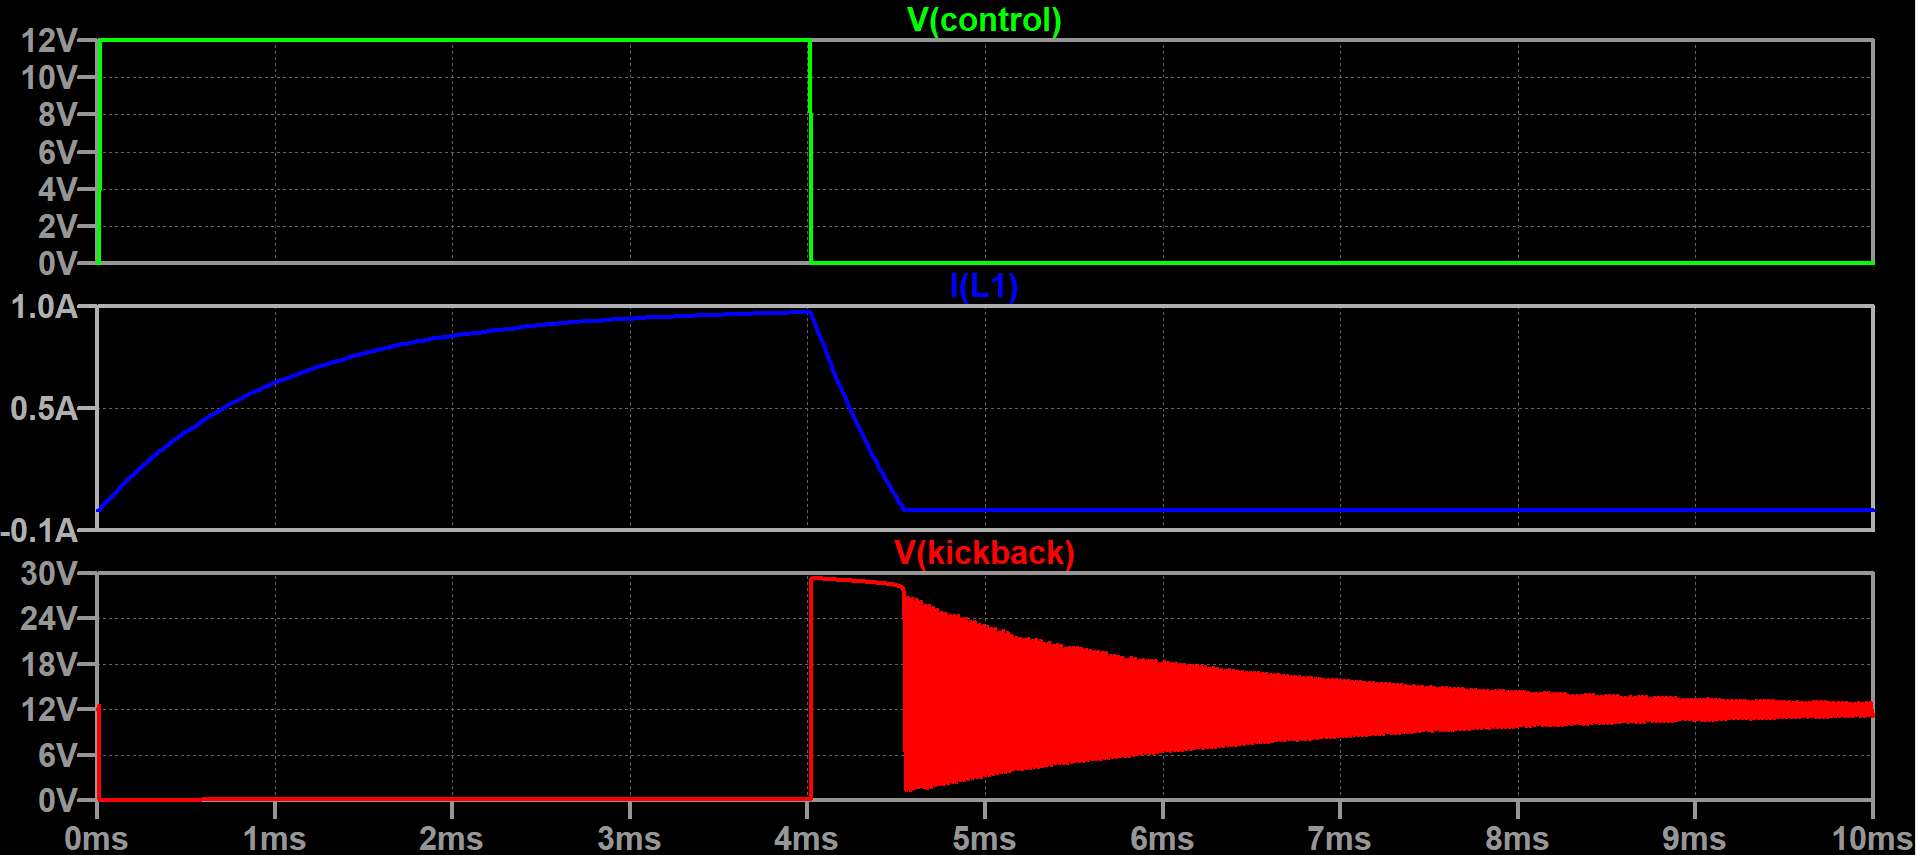
\includegraphics[width=\textwidth]{zener_diode_sim_results.png}
                        \caption{Simulated waveforms showing inductor current and voltage}
                        \label{fig:zener_waveform}
                    \end{subfigure}
                    \caption{Zener diode implementation for inductive kickback protection. The Zener diode clamps the voltage spike, protecting the MOSFET from high voltages.}
                    \label{fig:zener_combined}
                \end{figure}

                For the prototype, the Zener approach was chosen. Care must be taken when choosing MOSFETs and Zener diodes to ensure that the Zener clamp voltage won't overcome the MOSFET's rated breakdown voltage, which could lead to catastrophic failure of the driver circuit.

                %% The circuit was also designed to be normally open, that is, the output will be low by default, so in case of failure, the output will be low, which means the injectors stay closed. \gls{tvs} diodes are also used to protect the input from overvoltage spikes, as well as the \gls{mcu} from the inductive kickback. A voltage follower circuit was also added to the \gls{mcu} outputs to guarantee isolation between logic and power circuits, preventing the high currents from affecting the \gls{mcu} operation.
%% 
                %% Later, input optical isolation had to be added to the circuit. The "Easy - U1 WEBER" \gls{ecu} uses an isolated ground for the injectors, not connected to the battery ground. This means that the input signals from the \gls{ecu} must be isolated from the output signals to prevent ground loops and ensure proper operation. An optocoupler was added to the input side of the circuit to provide this isolation, at the cost of increased complexity and latency (in the microsecond range, still very tolerable for the application).

            \subsubsection{FET Ringing Mitigation}

                As can be seen in figure \ref{fig:zener_waveform}, when increasing the clamping voltage, the ringing of the MOSFET gate can become more pronounced, resulting in severe ringing on the output, visible in the voltage waveform. According to the Toshiba Electronics application note on the topic \autocite{toshibaelectronicdevices&storagecorporationParasiticOscillationRinging}, when the FET turns off, the di/dt of the drain current over the stray inductances causes a voltage surge at the drain and source. This surge voltage is given by \autocite{toshibaelectronicdevices&storagecorporationParasiticOscillationRinging}:

                \begin{equation}
                V_{\text{Surge}} = L_{S_2} \times \frac{di}{dt}
                \end{equation}

                When the diode in the drain-source loop is in conduction (i.e., energy from L is being recirculated), the circuit causes ringing since the surge voltage resonates with the $C_{ds}$ of the MOSFET and the stray inductance $L_{S2}$ \autocite{toshibaelectronicdevices&storagecorporationParasiticOscillationRinging}. Since the impedance of C1 is sufficiently low for parasitic oscillation frequency, it can be considered to be short-circuited \autocite{toshibaelectronicdevices&storagecorporationParasiticOscillationRinging}.

                The surge voltage is superimposed on the $v_{GS}$ voltage via the gate-drain capacitance $C_{gd}$ of the MOSFET. As a result, it might also affect the gate inductance as shown in Figure \ref{fig:ringing_mitigation}, and result in the ringing of the gate voltage \autocite{toshibaelectronicdevices&storagecorporationParasiticOscillationRinging}.

                \begin{figure}[H]
                    \centering
                    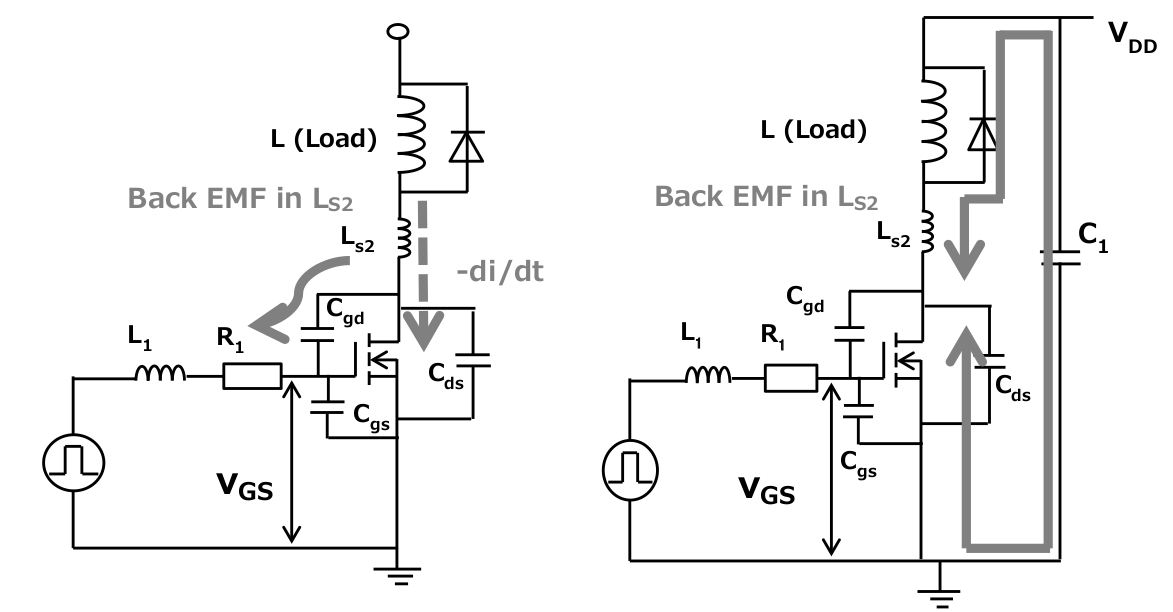
\includegraphics[width=0.8\textwidth]{fet_ringing_toshiba.png}
                    \caption{Positive Feedback Paths when Driving Inductances. Adapted from \autocite{toshibaelectronicdevices&storagecorporationParasiticOscillationRinging}}
                    \label{fig:ringing_mitigation}
                \end{figure}

                This FET ringing can be mitigated in several ways \autocite{toshibaelectronicdevices&storagecorporationParasiticOscillationRinging}. For this application, a simple gate resistor was used, which will limit the di/dt of the gate voltage, at the cost of a slightly slower turn-on time of the MOSFET \autocite{toshibaelectronicdevices&storagecorporationParasiticOscillationRinging}.

                %% include single picture with the simulation results of the resistor
                \begin{figure}[H]
                    \centering
                    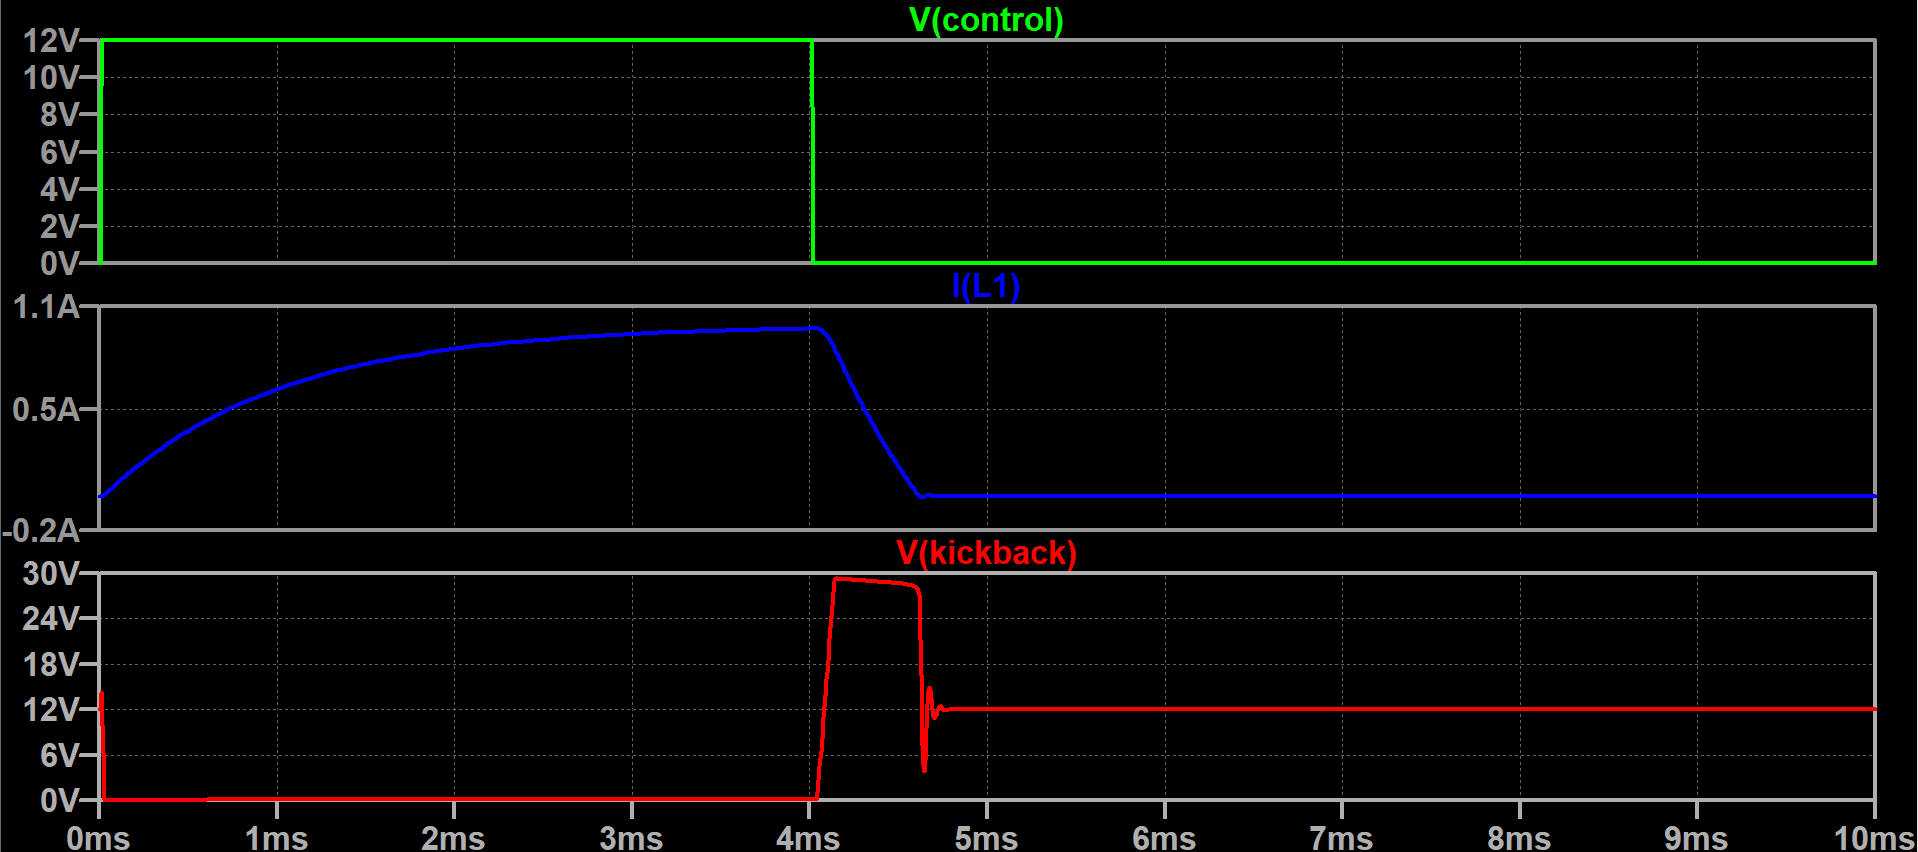
\includegraphics[width=0.8\textwidth]{decreased_ringing_sim_results.png}
                    \caption{Simulation results with the added gate resistance: reduced ringing.}
                    \label{fig:gate_resistor_simulation}
                \end{figure}

                The proposed solution was designed with SPICE, and later validated on the real hardware.


    \section{Prototype Construction}

        A custom two-sided PCB was designed in KiCad to accommodate all the output driver components. The PCB was designed with a double-sided layout, with both a ground plane and a power plane for noise rejection purposes. A small optical isolation board was hand-soldered, along with a development board for the \gls{mcu}. The reason for separating the system into several boards was to allow for easier replacement of parts in case of failure, and more adaptability. The complete system block diagram can be seen in figure \ref{fig:complete_system_block_diagram}.

        The prototype boards were also pre-assembled by the PCB manufacturer. Due to the MOSFETs operating in PWM mode only, thermal dissipation is not a problem, and no heat sinks were required.

        A prototype system for the two-cylinder Weber motor was assembled in a small enclosure, with the injector driver, power supply, \gls{mcu} and a potentiometer to adjust the \gls{injection_pulse_width} extension rate. Later, the optical isolation module was assembled on a prototype board, also added to the enclosure.

        %% insert figure with the complete system block diagram
        \begin{figure}[H]
            \centering
            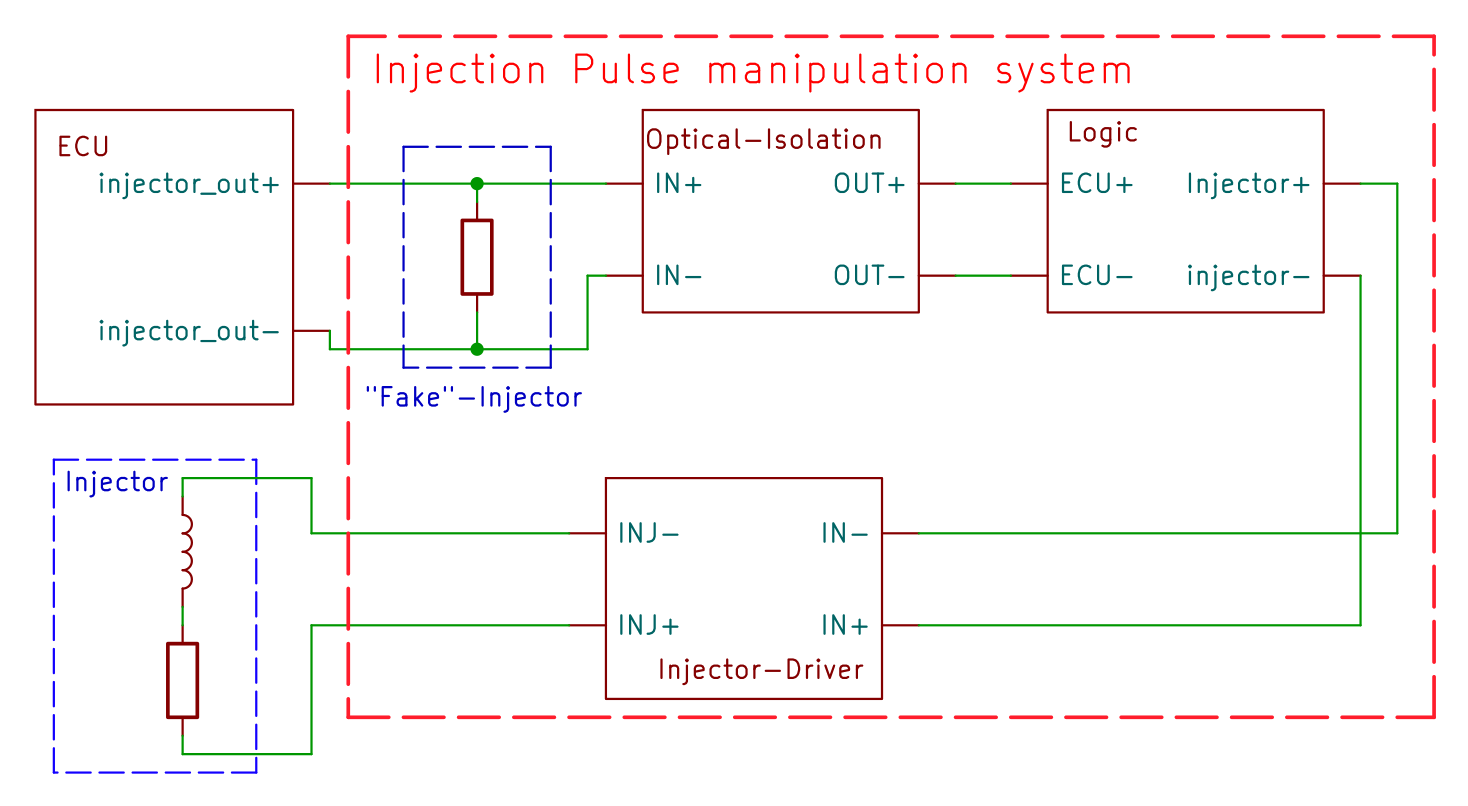
\includegraphics[width=0.8\textwidth]{complete_system_diagram.png}
            \caption{Complete System Block Diagram}
            \label{fig:complete_system_block_diagram}
        \end{figure}

        \begin{figure}[H]
            \centering
            \begin{subfigure}{0.4\textwidth}
                \centering
                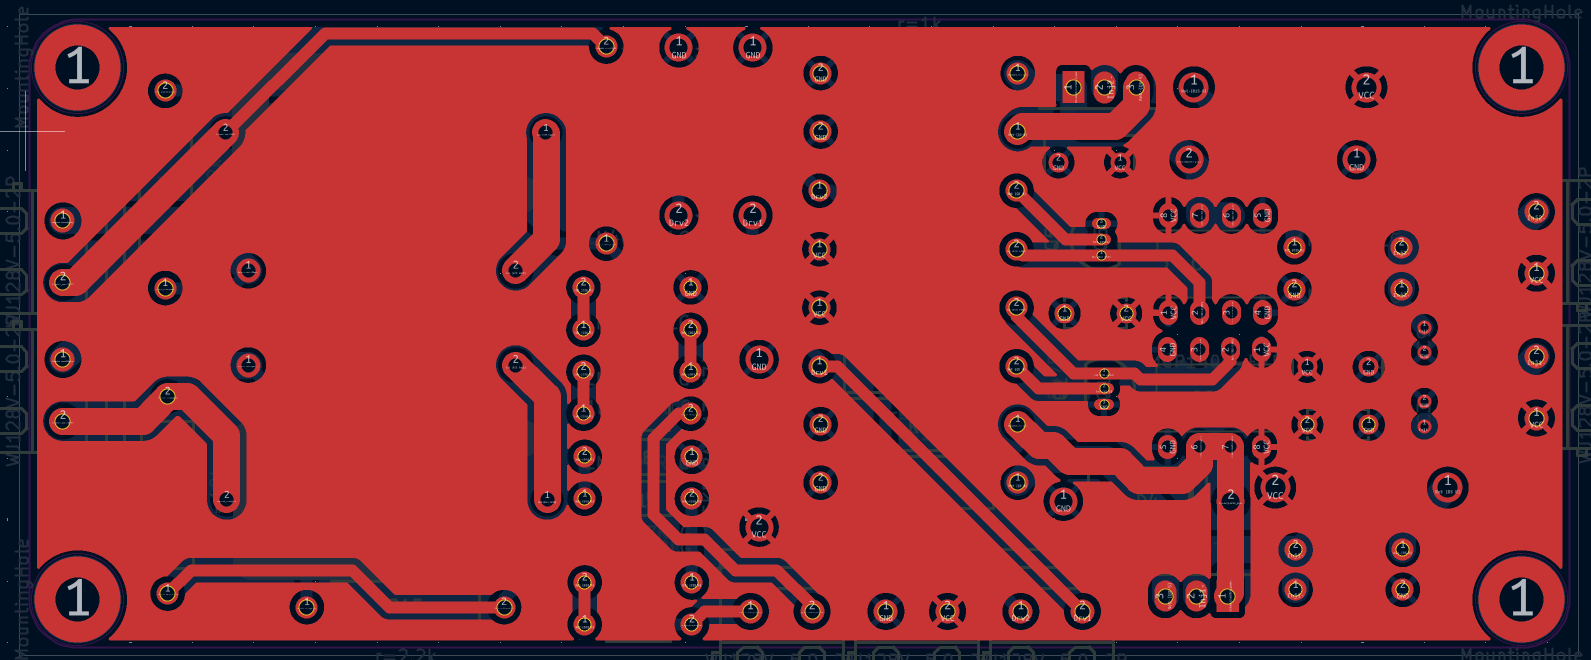
\includegraphics[width=\textwidth]{PH_board_back.png}
                \caption{Injector Driver Back Copper}
                \label{fig:pcb_back}
            \end{subfigure}
            \hfill
            \begin{subfigure}{0.4\textwidth}
                \centering
                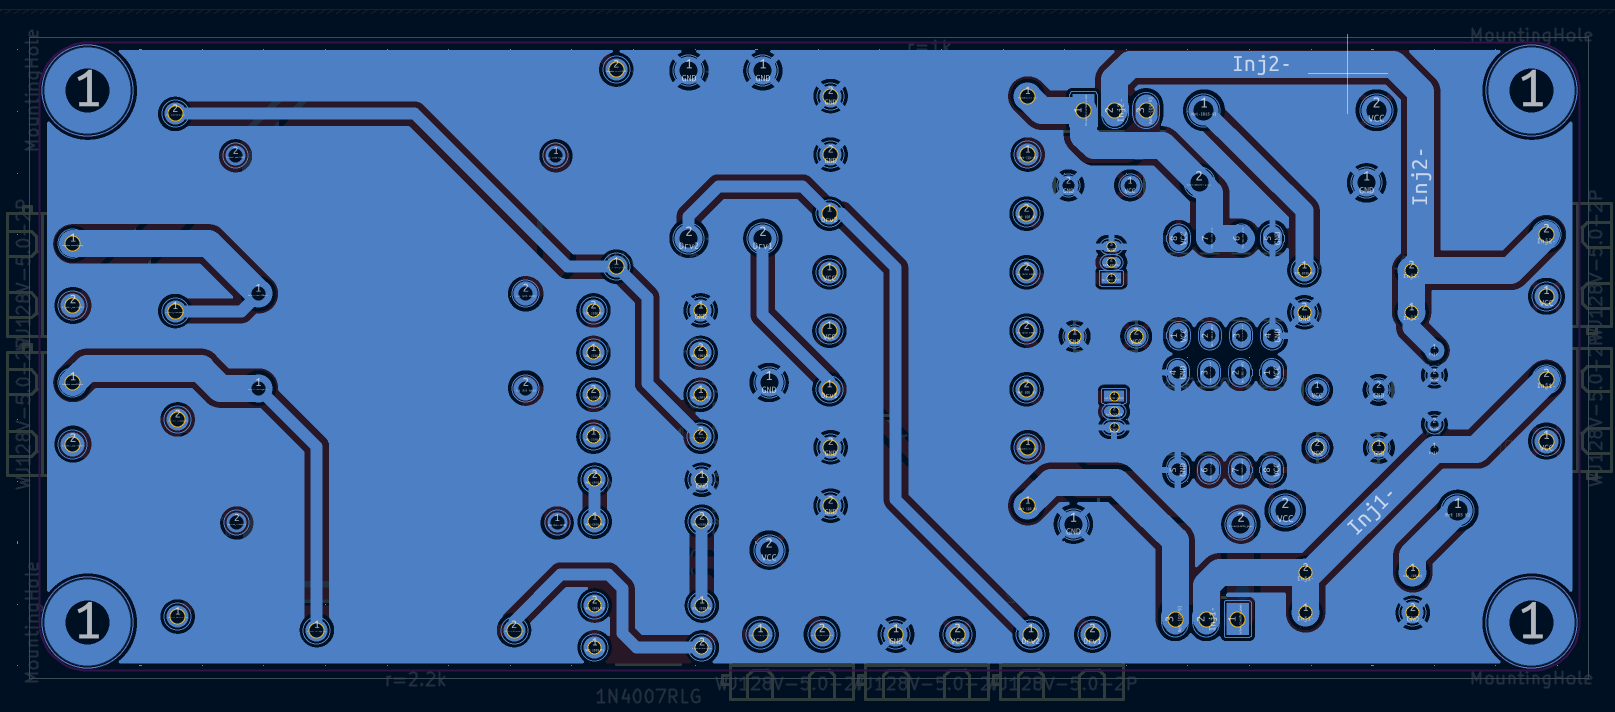
\includegraphics[width=\textwidth]{PH_board_front.png}
                \caption{Front Copper}
                \label{fig:pcb_front}
            \end{subfigure}
            \hfill
            \begin{subfigure}{0.37\textwidth}
                \centering
                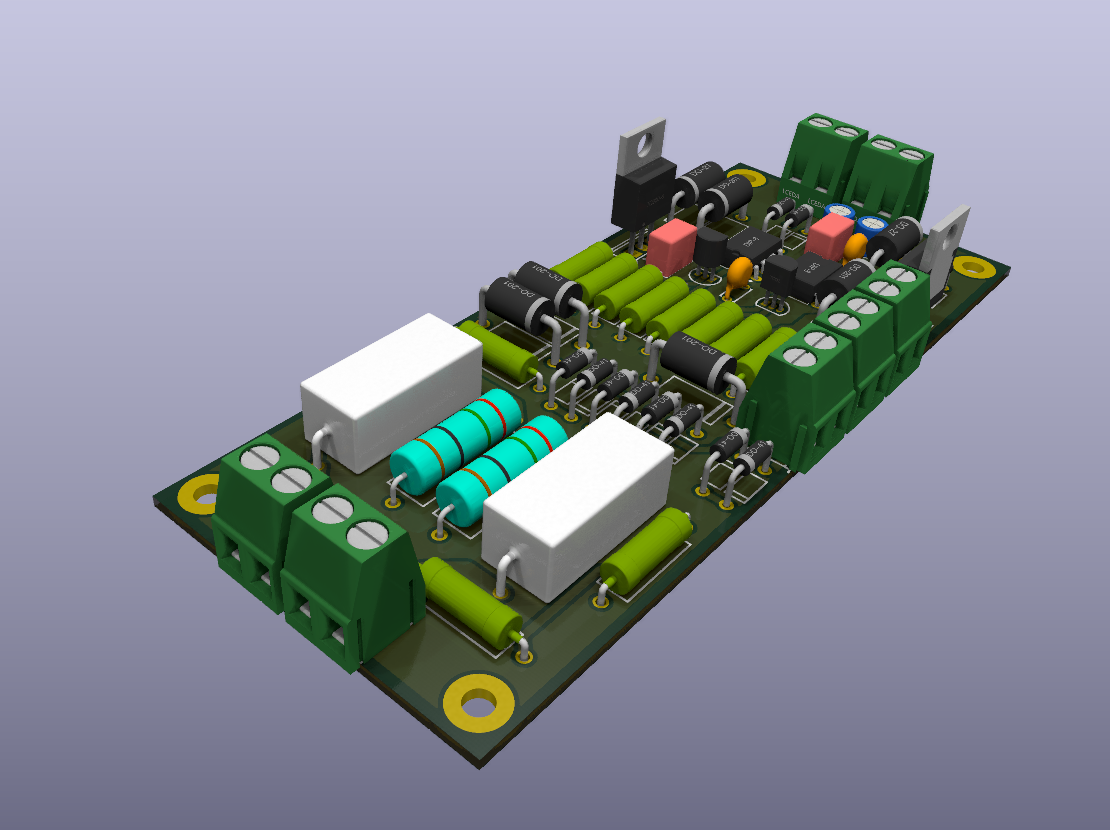
\includegraphics[width=\textwidth]{PH_board_3d.png}
                \caption{Driver Module 3D Render}
                \label{fig:pcb_3d}
            \end{subfigure}
            \hfill
             \begin{subfigure}{0.4\textwidth}
                \centering
                \includegraphics[width=\textwidth]{module_closed_top.jpg}
                \caption{Complete System}
                \label{fig:module_ready}
            \end{subfigure}
            \caption{PCB Design for the Peak and Hold Injector Driver: (a) Back copper layer with short traces for high current paths, (b) Front copper layer with control circuitry, (c) 3D rendered view showing component placement (d), Enclosure with all components ready to be mounted on the motor}
            \label{fig:pcb_design}
        \end{figure}






